\def \figmap {
\begin{figure*}
\centering
\includegraphics[scale=1.0]{m31flux-figures/map_full.pdf}
\caption[PHAT survey map.]{Map of the PHAT survey area. The 21 PHAT bricks
    analyzed in this study are outlined and numbered. Each brick was divided
    into 450 regions on a $15 \times 30$ grid, as shown for brick 2 in the
    inset panel. \citet{Lewis:2014} derived the \sfh{s} for all of the $\sim
    24\aarcsec \times 27\aarcsec$ regions.
}
\label{fig:map}
\end{figure*}
}


\def \figmodfluxmapsfuv {
\begin{figure*}
\centering
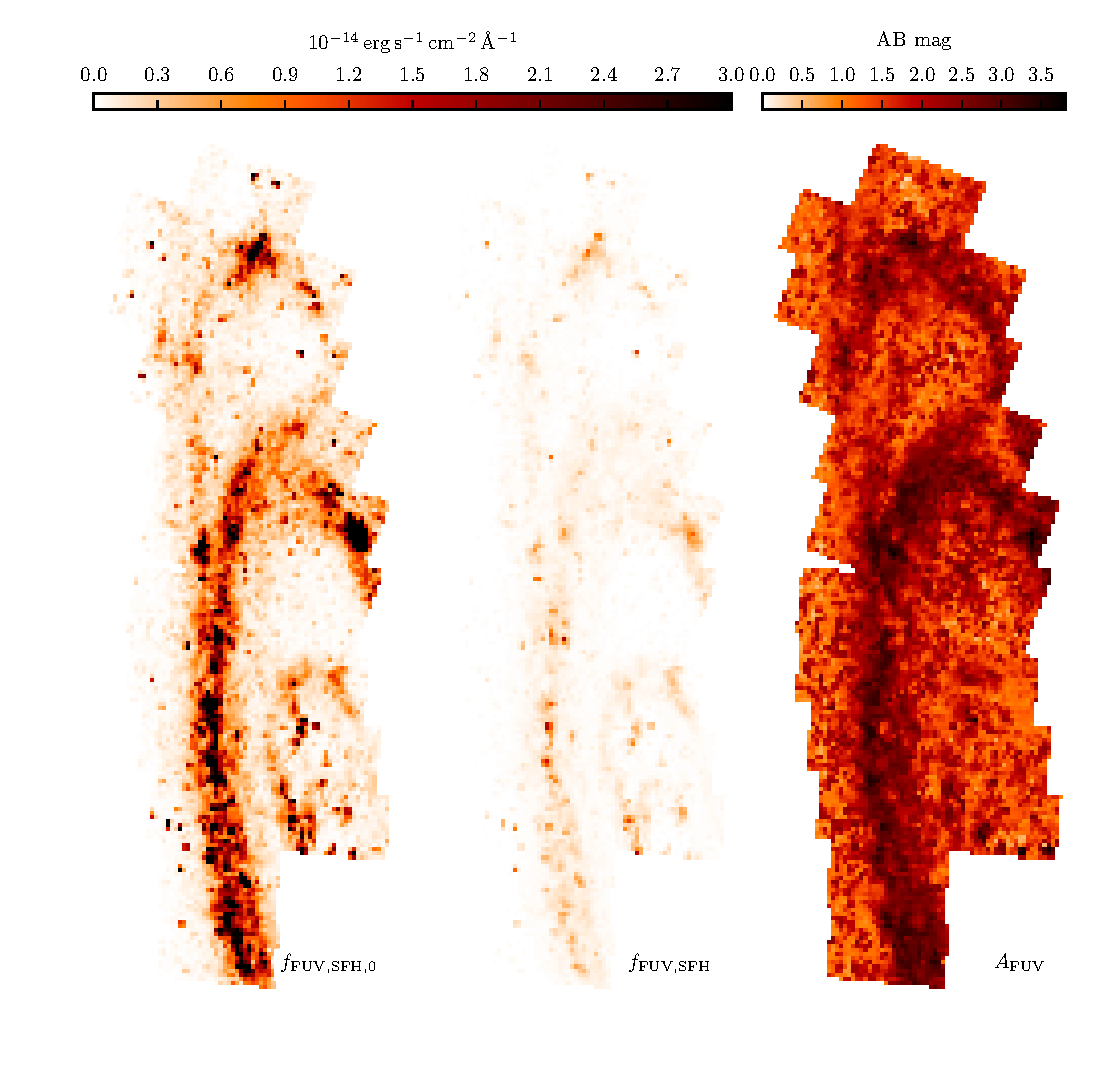
\includegraphics[width=\textwidth]{m31flux-figures/modfluxmaps_fuv.pdf}
\caption[\fuv{} flux map modeled from the \sfh{s}.]{\fuv{} flux modeled from
    the \sfh{s}. The intrinsic flux, \ffuvsfhz{}, is shown in the left panel
    and the middle panel shows the flux attenuated according to the extinction
    model, \ffuvsfh{} (also shown alongside the observed GALEX \fuv{} flux in
    Figure \ref{fig:fluxmapsfuv}). The \fuv{} extinction, \afuv{}, derived
    from \ffuvsfhz{} and \ffuvsfh{} is shown on the right.
}
\label{fig:modfluxmapsfuv}
\end{figure*}
}


\def \figmodfluxmapsnuv {
\begin{figure*}
\centering
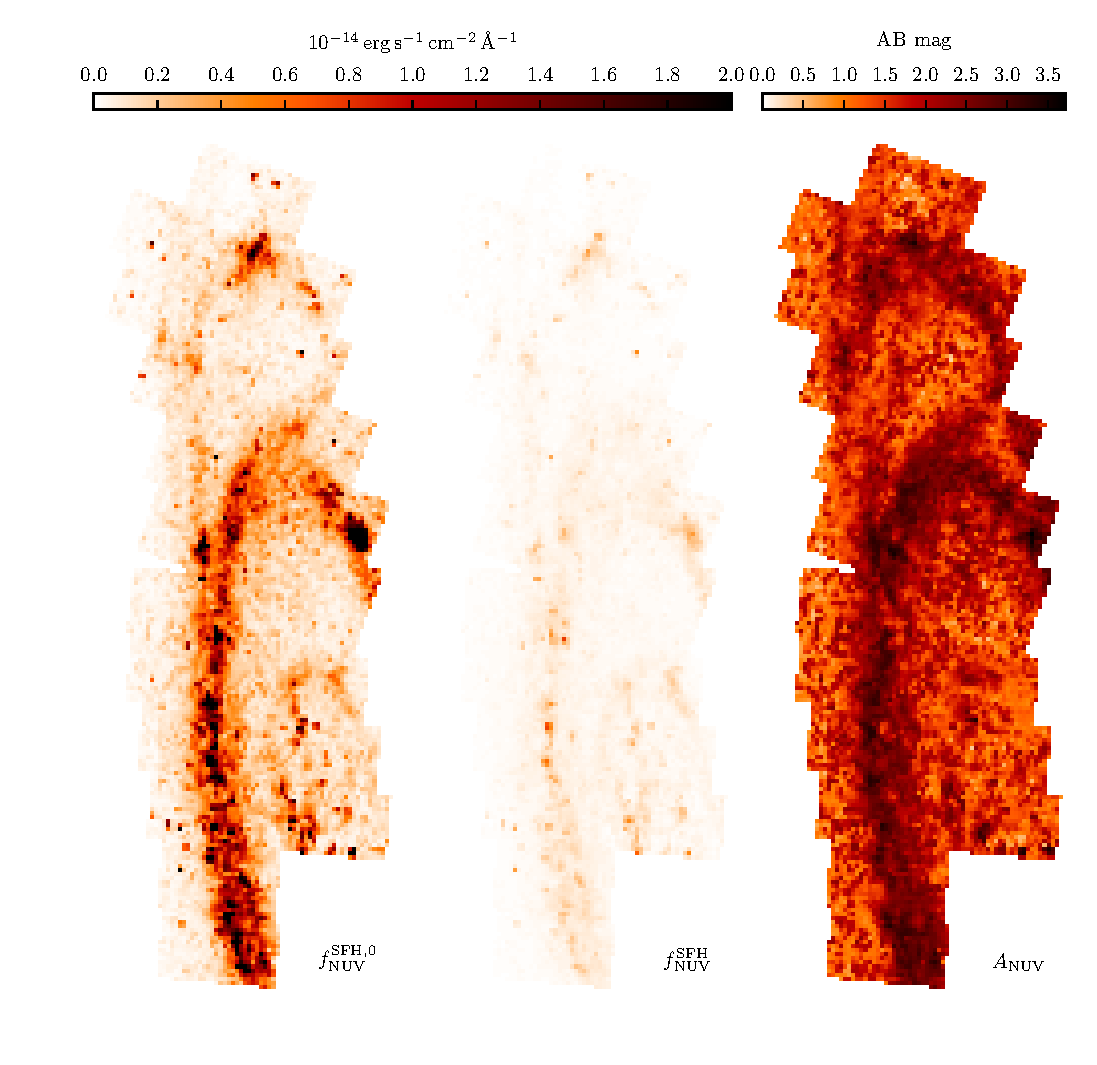
\includegraphics[width=\textwidth]{m31flux-figures/modfluxmaps_nuv.pdf}
\caption[\nuv{} flux map modeled from the \sfh{s}.]{Same as Figure
    \ref{fig:modfluxmapsfuv}, but for the \nuv{} filter.
}
\label{fig:modfluxmapsnuv}
\end{figure*}
}


\def \figfluxmapsfuv {
\begin{figure*}
\centering
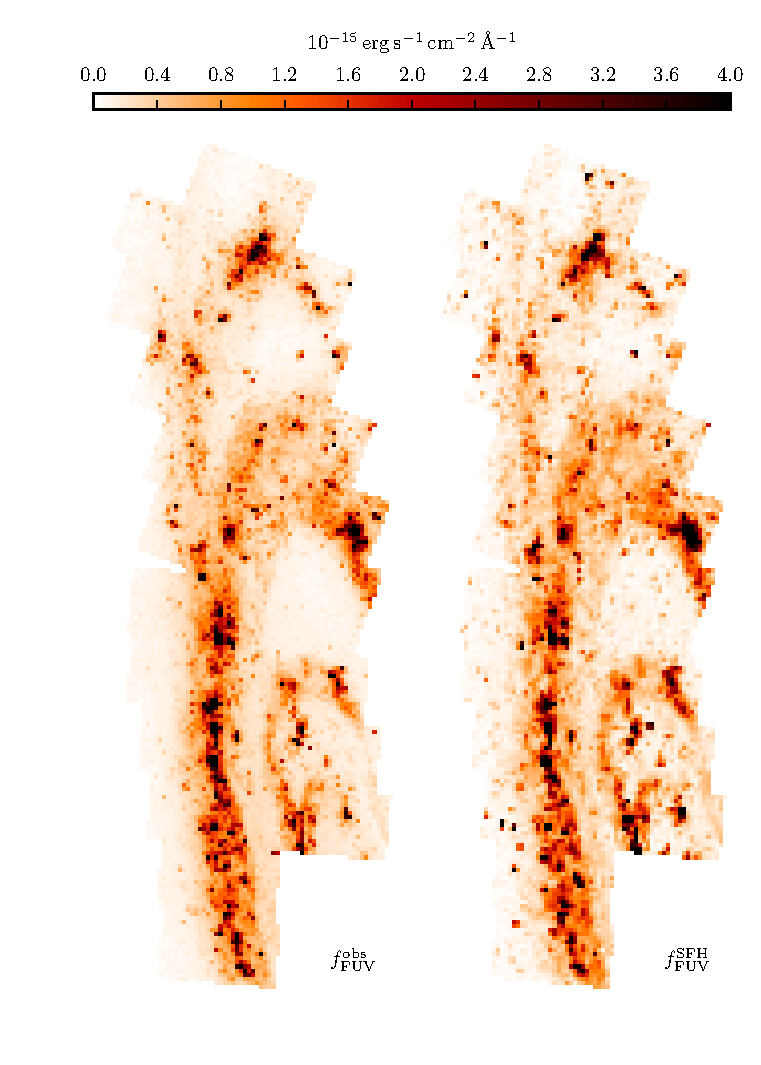
\includegraphics[scale=0.9]{m31flux-figures/fluxmaps_fuv.pdf}
\caption[Observed and synthetic attenuated \fuv{} flux maps.]{Observed \fuv{}
    flux from GALEX, \ffuvobs{} (left), and synthetic attenuated \fuv{} flux
    from the \sfh{s}, \ffuvsfh{} (right). The observed map has been clipped to
    the PHAT survey border to match the synthetic map. The synthetic fluxes
    show excellent morphological agreement with the observed fluxes.
}
\label{fig:fluxmapsfuv}
\end{figure*}
}


\def \figfluxmapsnuv {
\begin{figure*}
\centering
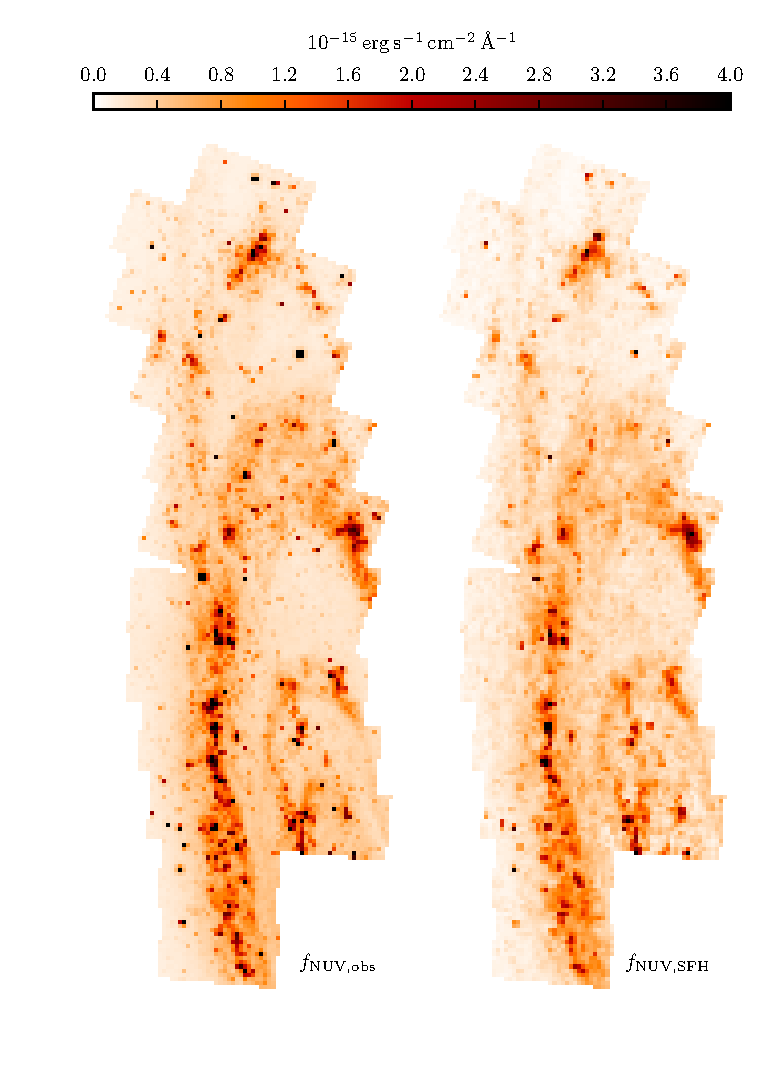
\includegraphics[scale=0.9]{m31flux-figures/fluxmaps_nuv.pdf}
\caption[Observed and synthetic attenuated \nuv{} flux maps.]{Same as Figure
    \ref{fig:fluxmapsfuv}, but for the \nuv{} filter.
}
\label{fig:fluxmapsnuv}
\end{figure*}
}


\def \figsfrmapsone {
\begin{figure*}
\centering
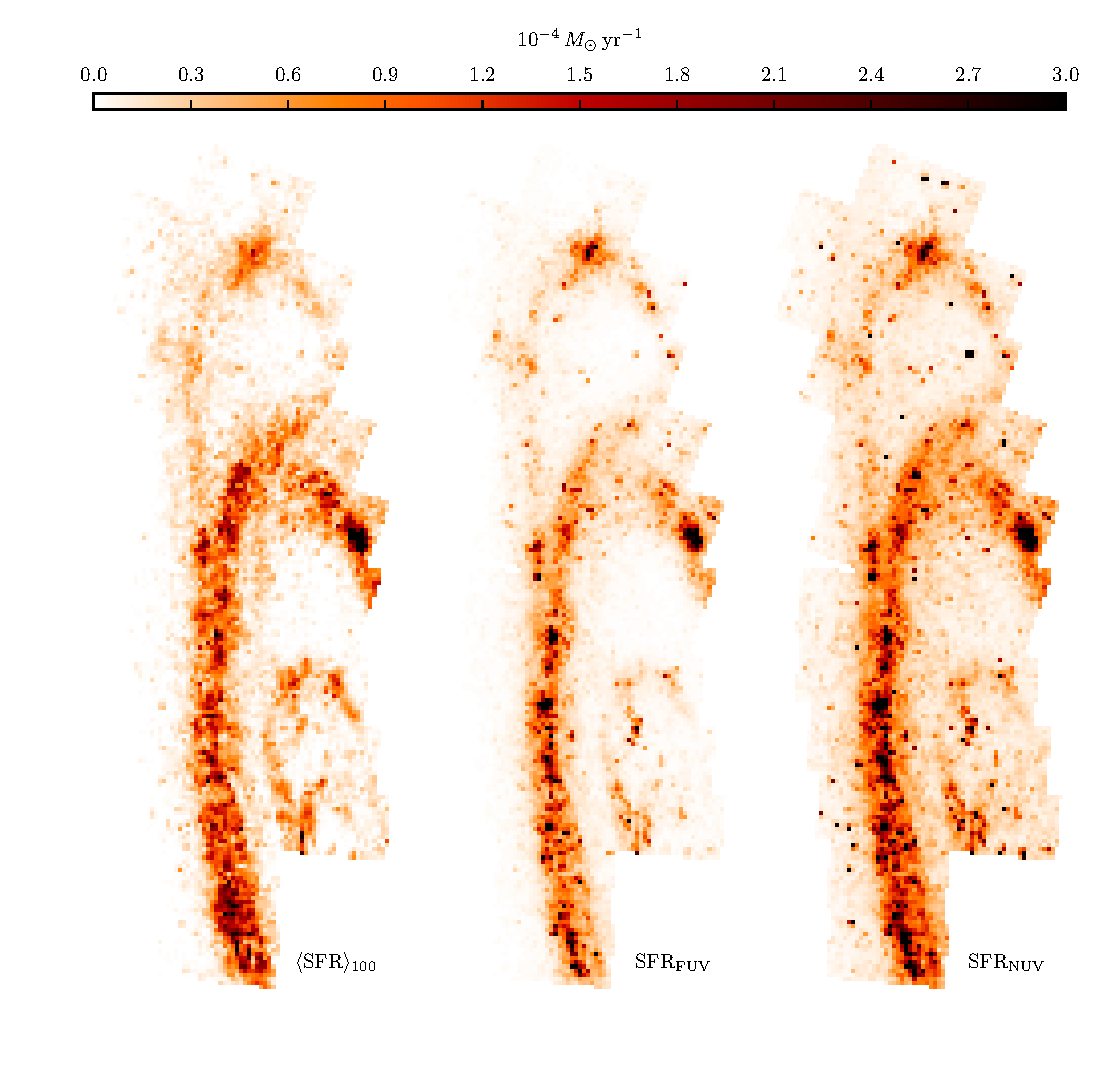
\includegraphics[width=\textwidth]{m31flux-figures/sfrmaps1.pdf}
\caption[\sfr{} maps from estimates based on observed fluxes compared with the
mean \sfr{} map from the \sfh{s}.]{\fuv{} and \nuv{} flux-based \sfr{s},
    \sfrfuv{} (middle) and \sfrnuv{} (right), compared with \sfroneh{} (left),
    the mean \sfr{} over the last $100\myr$ of the \sfh{s}. The flux-based
    \sfr{s} were derived from the observed GALEX fluxes, \fuvobs{} and
    \nuvobs{} (Figures \ref{fig:fluxmapsfuv} and \ref{fig:fluxmapsnuv}),
    corrected for extinction using \afuv{} and \anuv{} (Figures
    \ref{fig:modfluxmapsfuv} and \ref{fig:modfluxmapsnuv}). The \sfr{} maps
    show good overall agreement.
}
\label{fig:sfrmapsone}
\end{figure*}
}


\def \figsfrmapstwo {
\begin{figure*}
\centering
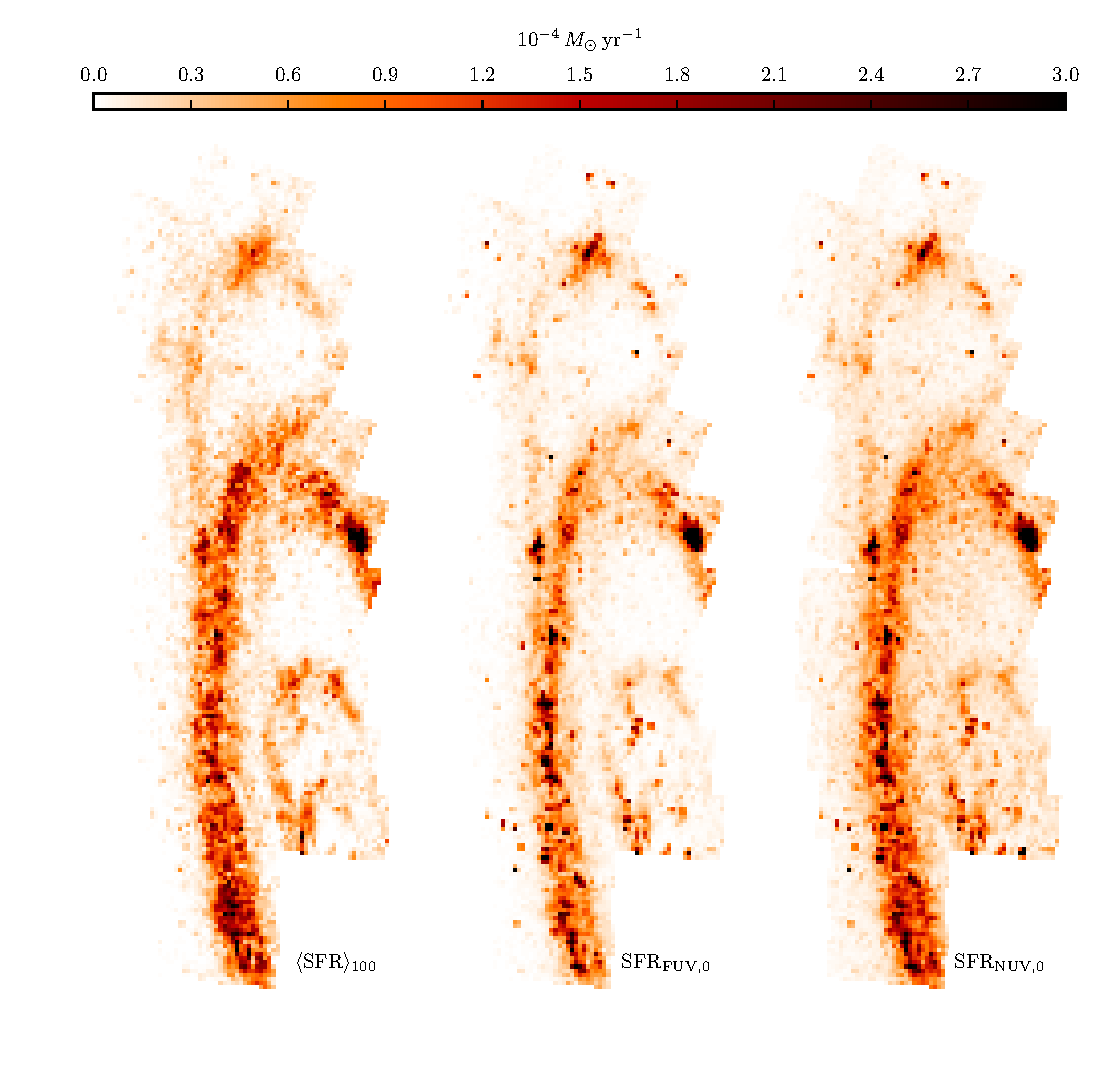
\includegraphics[width=\textwidth]{m31flux-figures/sfrmaps2.pdf}
\caption[\sfr{} maps from estimates based on synthetic intrinsic fluxes
compared with the mean \sfr{} map from the \sfh{s}.]{Same as Figure
    \ref{fig:sfrmapsone}, but instead comparing \sfroneh{} with \sfrfuvz{} and
    \sfrnuvz{}, the \sfr{s} from the synthetic intrinsic (i.e., unattenuated)
    fluxes from Figures \ref{fig:modfluxmapsfuv} and \ref{fig:modfluxmapsnuv}.
    The synthetic intrinsic fluxes were derived assuming a fully populated IMF
    so there is no inconsistency with the flux calibration, which assumes the
    same. Like the \sfr{s} based on observed flux, these \sfr{s} also show good
    agreement with \sfroneh{}.
}
\label{fig:sfrmapstwo}
\end{figure*}
}


\def \figfuvfluxratio {
\begin{figure*}
\centering
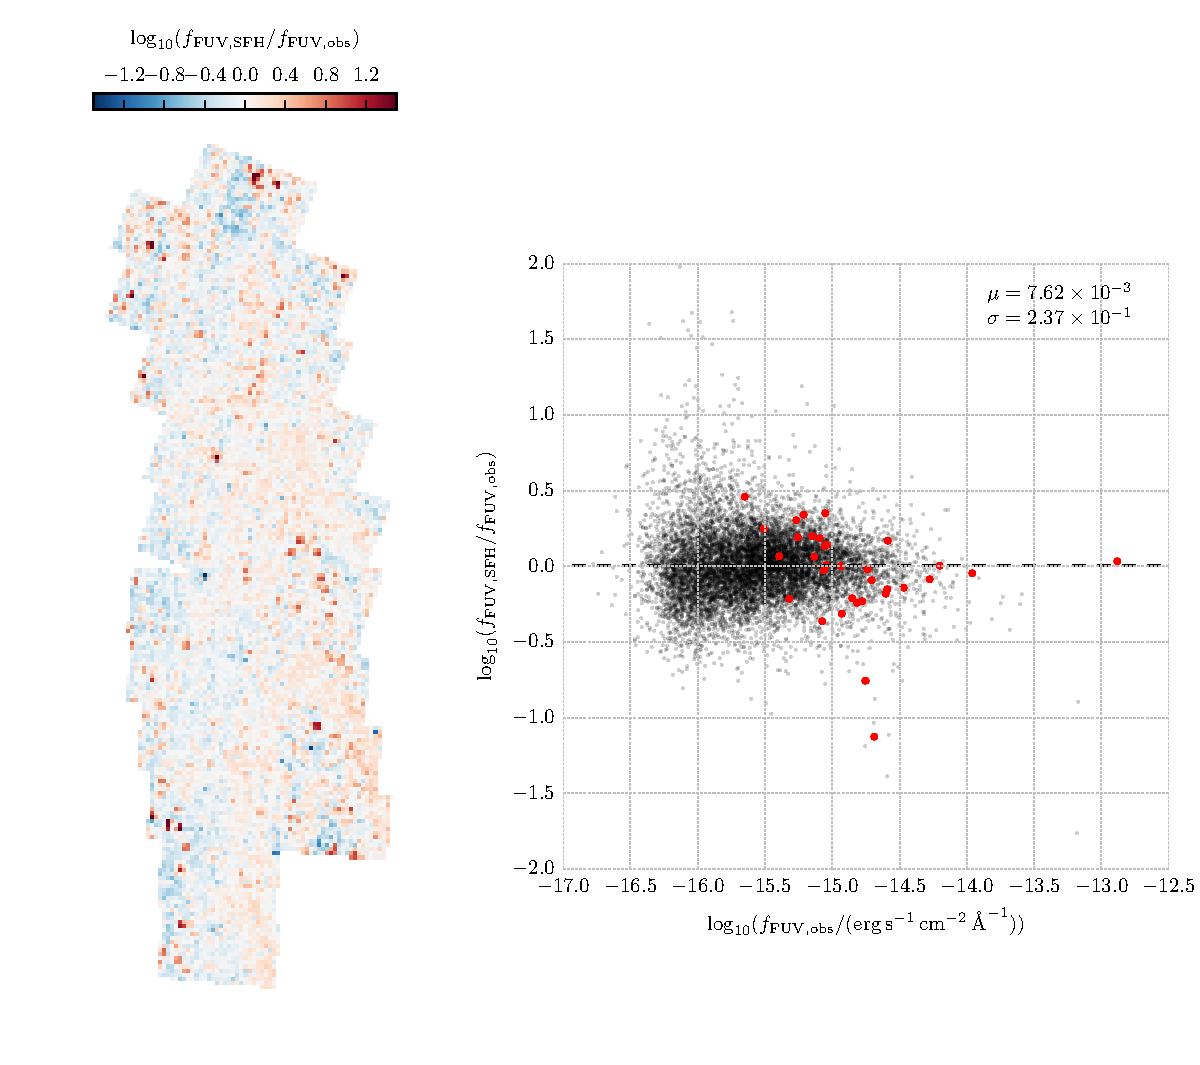
\includegraphics[width=\textwidth]{m31flux-figures/flux_fuv_sfh-vs-obs.pdf}
\caption[Ratio of the synthetic flux to the observed flux in the \fuv{}
filter.]{Ratio of the synthetic attenuated flux, \ffuvsfh{}, to the GALEX
    observed flux, \ffuvobs{}, in the \fuv{} filter. The log flux ratios in the
    scatter plot follow a normal distribution with $\mu = 7.62\times 10^{-3}$
    (horizontal dashed line) and $\sigma = 2.37\times 10^{-1}$. The median
    ratio is 1.02 with 68\% confidence limits of 0.59 and 1.76. \ffuvsfh{} and
    \ffuvobs{} are therefore consistent on average. The flux ratio variance
    increases with decreasing observed flux, suggesting that the uncertainties
    are dominated by incomplete IMF sampling. The large red circles represent
    flux ratios for the UV-bright regions from \citet{Simones:2014} and are
    consistent with the main sample. The map shows a fairly even spatial
    distribution for the flux ratios, with the most severely overestimated and
    underestimated pixels occurring primarily in the faint, off-arm areas of
    the galaxy, as shown in the scatter plot.
}
\label{fig:fuvfluxratio}
\end{figure*}
}


\def \fignuvfluxratio {
\begin{figure*}
\centering
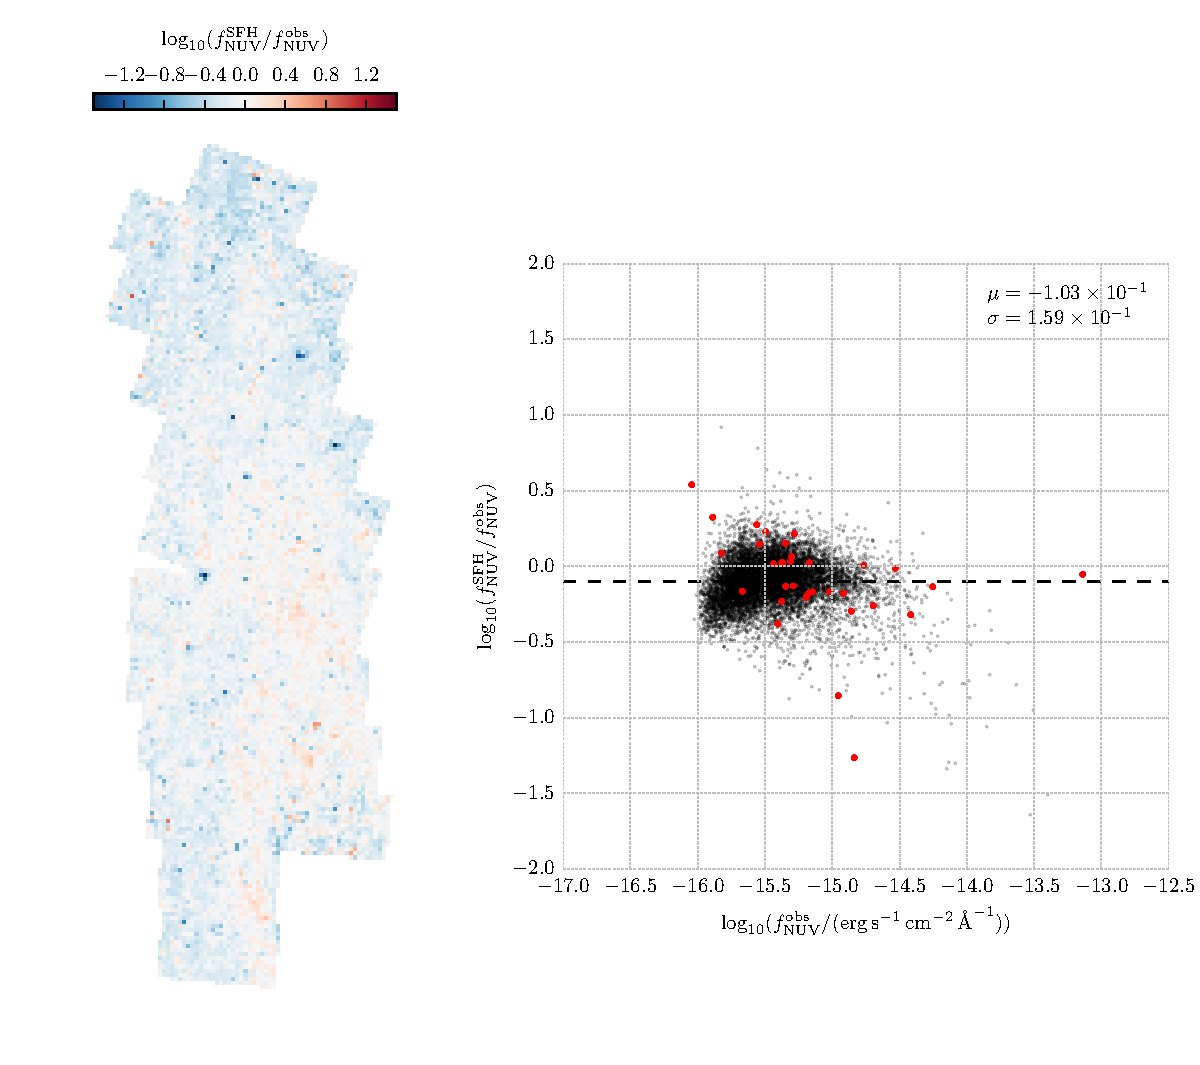
\includegraphics[width=\textwidth]{m31flux-figures/flux_nuv_sfh-vs-obs.pdf}
\caption[Ratio of the synthetic flux to the observed flux in the \nuv{}
filter.]{Same as Figure \ref{fig:fuvfluxratio}, but for the \nuv{} filter. In
    this case, the log-normal distribution is characterized by $\mu =
    -1.03\times 10^{-1}$ and $\sigma = 1.59\times 10^{-1}$. The median ratio is
    0.79 with 68\% confidence limits of 0.55 and 1.14. \fnuvsfh{} and
    \fnuvobs{} are therefore consistent on average. The role of IMF sampling is
    not as important for \fnuvobs{}, so the uncertainties in \fnuvsfh{} are
    somewhat smaller.
}
\label{fig:nuvfluxratio}
\end{figure*}
}


\def \figfuvsfrratio {
\begin{figure*}
\centering
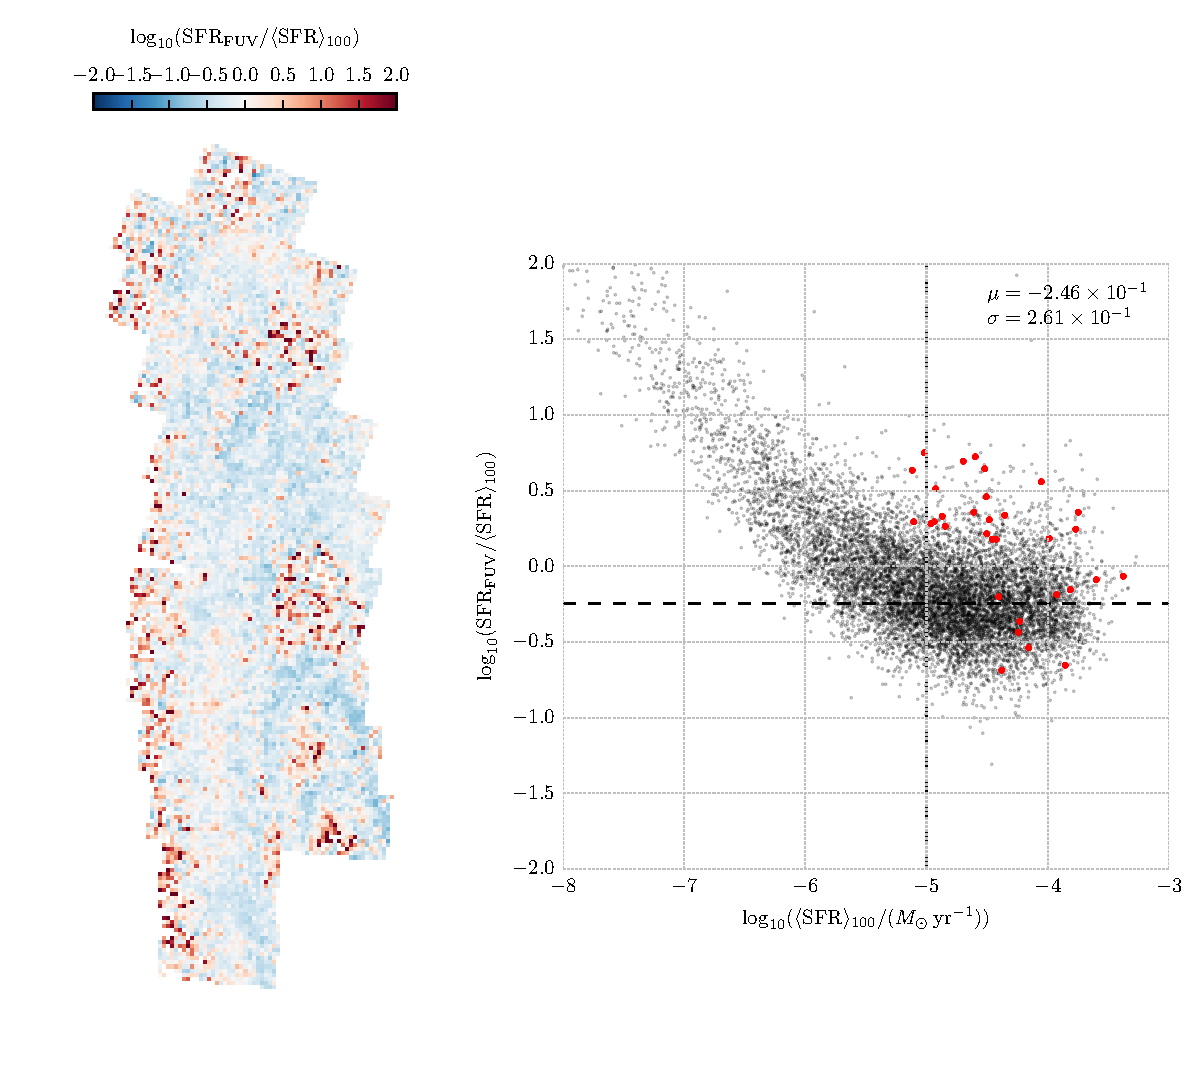
\includegraphics[width=\textwidth]{m31flux-figures/sfr_fuv-vs-mean.pdf}
\caption[Ratio of the \sfr{} based on the observed extinction-corrected \fuv{}
flux to the $100\myr$ mean \sfr{}.]{Ratio of the \sfr{} based on the observed
    extinction-corrected \fuv{} flux, \sfrfuv{}, to the $100\myr$ mean of the
    \sfh{}, \sfroneh{}. The log \sfr{} ratios show a linear tail feature with
    $-1$ slope and $-6.0$ intercept, implying that \sfrfuv{} becomes constant
    for $\sfroneh < 9.8\times 10^{-7}\msun\yr^{-1}$. We constrain our analysis
    to pixels with $\sfroneh10^{-5}\msun\yr^{-1}$ (vertical dashed line). Above
    this limit, the log \sfr{} ratios follow a normal distribution with $\mu =
    -2.46\times 10^{-1}$ (horizontal dashed line) and $\sigma = 2.61\times
    10^{-1}$. The median ratio is 0.57 with 68\% confidence limits of 0.31 and
    1.04, most likely due to incomplete IMF sampling. \sfrfuv{} and \sfroneh{}
    are therefore consistent on average. The large red circles represent \sfr{}
    ratios for the UV-bright regions from \citet{Simones:2014} and are
    consistent with the main sample. Apart from the faint, off-arm areas
    responsible for the tail feature, the map shows a fairly even spatial
    distribution for the \sfr{} ratios.
}
\label{fig:fuvsfrratio}
\end{figure*}
}


\def \fignuvsfrratio {
\begin{figure*}
\centering
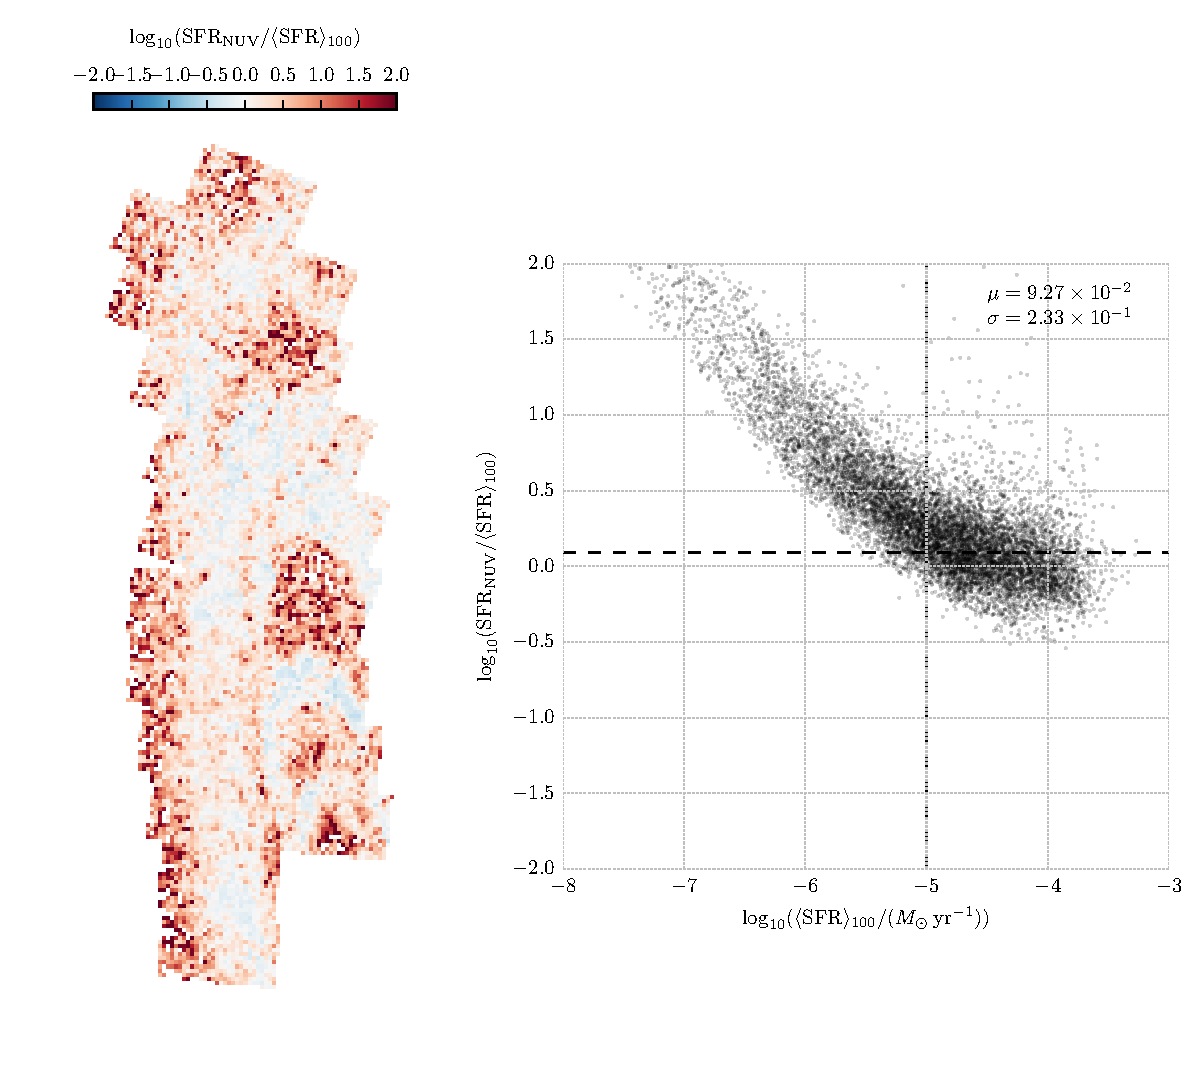
\includegraphics[width=\textwidth]{m31flux-figures/sfr_nuv-vs-mean.pdf}
\caption[Ratio of the \sfr{} based on the observed extinction-corrected \nuv{}
flux to the $100\myr$ mean \sfr{}.]{Same as Figure \ref{fig:fuvsfrratio}, but
    for the \nuv{} filter. In this case, the linear tail has an intercept of
    $-5.4$ such that \sfrnuv{} becomes constant for $\sfroneh < 4.1\times
    10^{-6}\msun\yr^{-1}$. The log-normal distribution is characterized by $\mu
    = 9.27\times 10^{-2}$ and $\sigma = 2.33\times 10^{-1}$. The median ratio
    is 1.24 with 68\% confidence limits of 0.72 and 2.12. \sfrnuv{} and
    \sfroneh{} are therefore consistent on average.
}
\label{fig:nuvsfrratio}
\end{figure*}
}


\def \figfuvzsfrratio {
\begin{figure*}
\centering
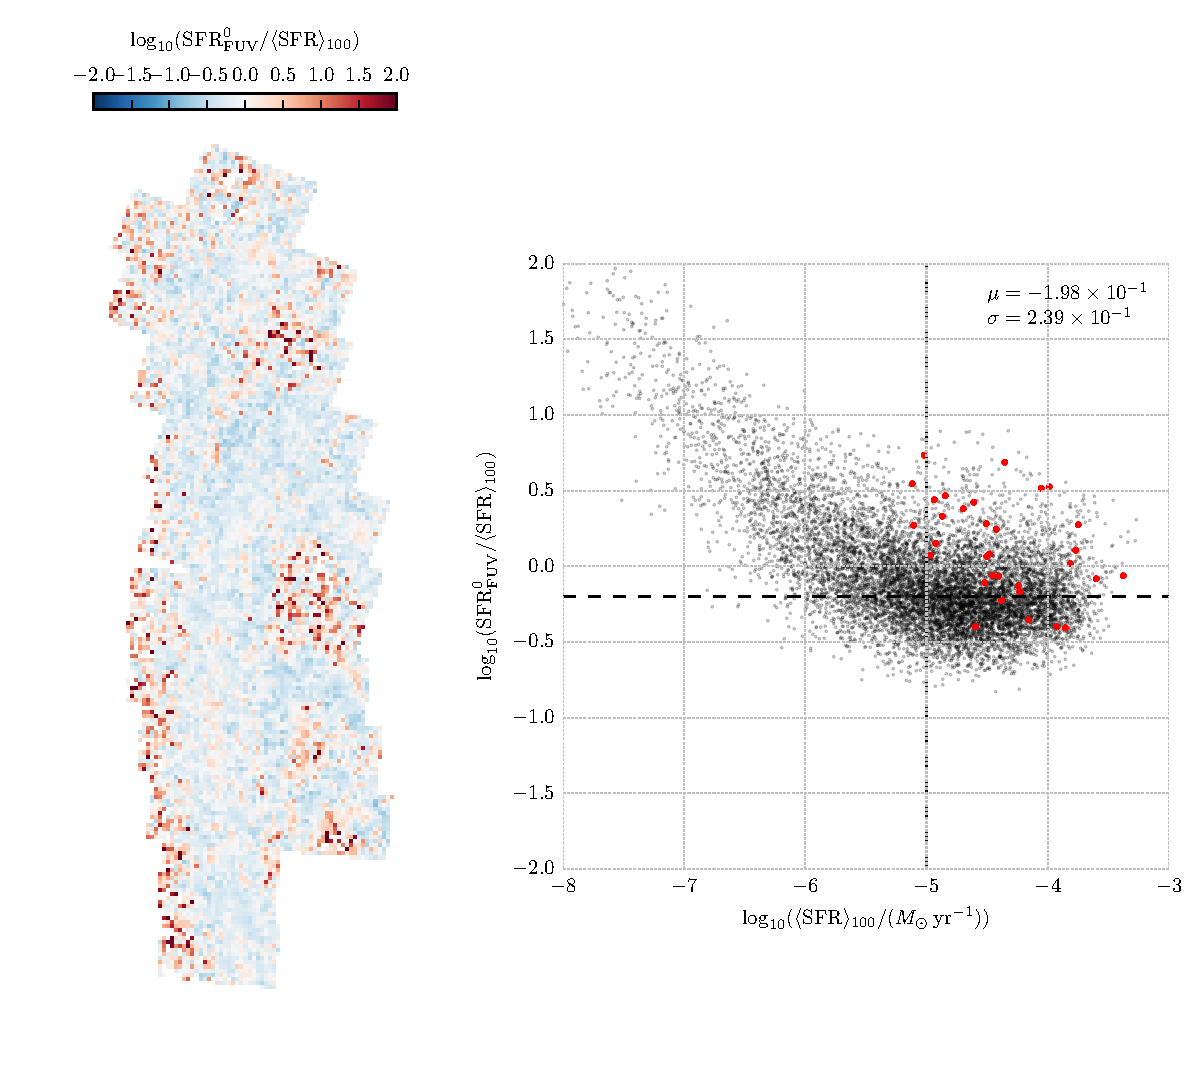
\includegraphics[width=\textwidth]{m31flux-figures/sfr_fuv0-vs-mean.pdf}
\caption[Ratio of the \sfr{} based on the synthetic intrinsic \fuv{} flux to
the $100\myr$ mean \sfr{}.]{Same as Figure \ref{fig:fuvsfrratio}, but based on
    synthetic instrinsic flux, \sfrfuvz{}. The log-normal distribution is
    characterized by $\mu = -1.98\times 10^{-1}$ and $\sigma = 2.39\times
    10^{-1}$. The median ratio is 0.63 with 68\% confidence limits of 0.37 and
    1.10. \sfrfuvz{} and \sfroneh{} are therefore consistent on average. The
    results here are similar to Figure \ref{fig:fuvsfrratio}, suggesting that
    \sfh{} variability does not significantly affect the \sfrfuv{}
    uncertainties.
}
\label{fig:fuvzsfrratio}
\end{figure*}
}


\def \fignuvzsfrratio {
\begin{figure*}
\centering
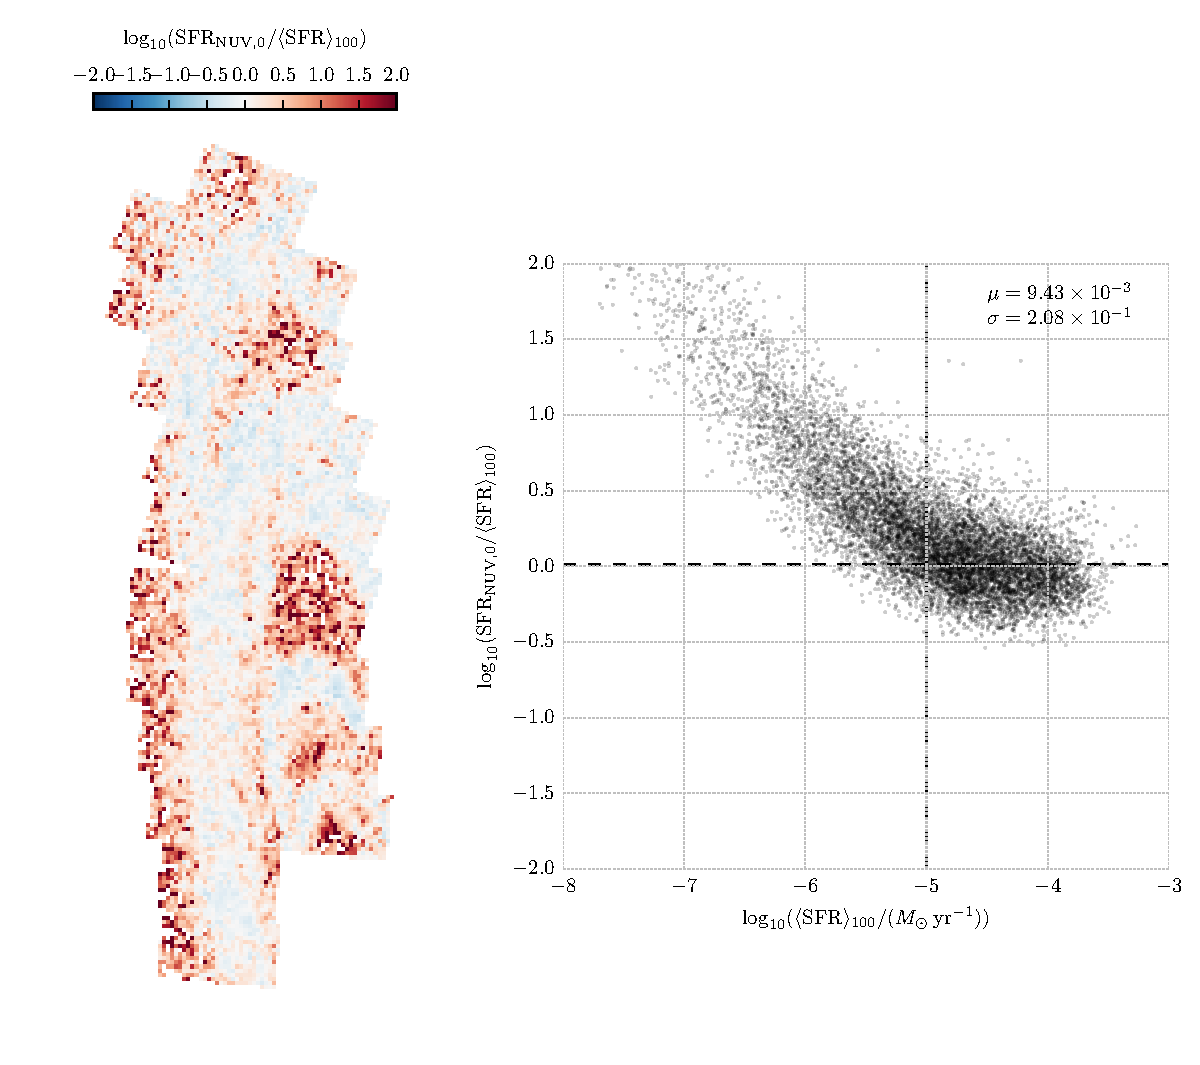
\includegraphics[width=\textwidth]{m31flux-figures/sfr_nuv0-vs-mean.pdf}
\caption[Ratio of the \sfr{} based on the synthetic intrinsic \nuv{} flux to
the $100\myr$ mean \sfr{}.]{Same as Figure \ref{fig:nuvsfrratio}, but based on
    synthetic instrinsic flux, \sfrnuvz{}. The log-normal distribution is
    characterized by $\mu = 9.43\times 10^{-3}$ and $\sigma = 2.08\times
    10^{-1}$. The median ratio is 1.02 with 68\% confidence limits of 0.63 and
    1.65. \sfrnuvz{} and \sfroneh{} are therefore consistent on average. The
    results here are similar to Figure \ref{fig:nuvsfrratio}, suggesting that
    \sfh{} variability does not significantly affect the \sfrnuv{}
    uncertainties.
}
\label{fig:nuvzsfrratio}
\end{figure*}
}




\def \tabfilters {
\begin{deluxetable*}{cccc}
\tabletypesize{\footnotesize}
\tablecaption{Filters and observations.\label{tab:mfx:filters}}
\tablewidth{0pt}
\tablehead{
    \colhead{Filter} &
    \colhead{$(\erg\ssec^{-1}\cm^{-2}\ang^{-1})/(\mathrm{counts}\ssec^{-1})$} &
    \colhead{AB mag zeropoint} &
    \colhead{Images}
}
\startdata
GALEX FUV &  $2.40 \times 10^{-15}\,\tablenotemark{a}$ &  18.82\tablenotemark{a} &  PS\_M31\_MOS00-fd-int.fits \\
          &                                            &                         &  PS\_M31\_MOS07-fd-int.fits \\
          &                                            &                         &  PS\_M31\_MOS08-fd-int.fits \\
          &                                            &                         &  PS\_M31\_MOS09-fd-int.fits \\
          &                                            &                         &  PS\_M31\_MOS10-fd-int.fits \\
GALEX NUV &  $2.06 \times 10^{-16}\,\tablenotemark{a}$ &  20.08\tablenotemark{a} &  PS\_M31\_MOS00-nd-int.fits \\
          &                                            &                         &  PS\_M31\_MOS07-nd-int.fits \\
          &                                            &                         &  PS\_M31\_MOS08-nd-int.fits \\
          &                                            &                         &  PS\_M31\_MOS09-nd-int.fits \\
          &                                            &                         &  PS\_M31\_MOS10-nd-int.fits
\enddata
\tablenotetext{a}{http://galexgi.gsfc.nasa.gov/docs/galex/FAQ/counts\_background.html}
\end{deluxetable*}

}
